\documentclass[9pt]{extarticle}
\usepackage[a4paper, total={6in, 8in}]{geometry}
\usepackage{tikz}
\usepackage{verbatim}
\usetikzlibrary{trees}

\title{NEA}
\author{Matthew Lugg}

\begin{document}

\maketitle

\newpage

\tableofcontents

\newpage

\section{Introduction}

Lazy evaluation is a computation model whereby all computations are deferred
until their results are required; this contrasts with eager evaluation, as used
by most conventional imperative languages. Lazy evaluation goes hand-in-hand
with functional programming, a programming paradigm based on Church's lambda
calculus rather than Turing machines. My goal is to write, in Haskell, a simple
compiler for a lazy, purely functional, strongly typed programming language
using the Hindley-Milner type system to amd64 assembly, which will allow for
simple Haskell-like programs to be written and compiled for modern CPUs.

\section{Analysis}

Haskell is generally considered the de-facto standard for lazy, purely
functional programming languages. It first appeared in 1990, and has been
extended over time to become a highly complex language today. Technically,
Haskell 2010 (the latest version of the language specification) is not
necessarily lazy, but non-strict. However, all popular implementations use lazy
semantics, so for all intents and purposes, Haskell can be considered a lazy
language. The most popular implementation is GHC, the Glasgow Haskell Compiler;
this compiler generates incredibly fast output assembly (often comparable in
speed to programs written in low-level languages like C) and supports over 100
language extensions for features such as GADTs and functional dependencies. 

There exist several other major purely functional languages, some of which
feature laziness. A prominent example is OCaml; however, this language differs
from Haskell in that it is eagerly evaluated by default and has opt-in lazy
semantics. Haskell is somewhat unique; as such, it may prove to be a major
source of inspiration for this project as the most similar existing solution. 

GHC's dialect of Haskell contains various sophisticated features with varying
levels of usage. Haskell, since its inception, contains typeclasses as a major
feature; these aid in the creation of polymorphic functions for things like
sorting. This is one of Haskell's most well-known and commonly-used features,
and as such, I would like to support this in my implementation; however, time
constraints will likely make this infeasible, as type inference and checking of
typeclasses is a relatively complex feature. 

\subsection{Parsing}

Parsing is an important part of any compiler; it is the translation of the
source code into a datatype known as an abstract syntax tree (AST); source code
is sometimes first converted into a ``concrete syntax tree'' instead, and then
into an AST, but this is relatively rare. As an example, in a conventional
imperative language, the expression \verb'f(x + y)' would parse into a tree like the
following:

\vspace{0.5cm}

\begin{center}
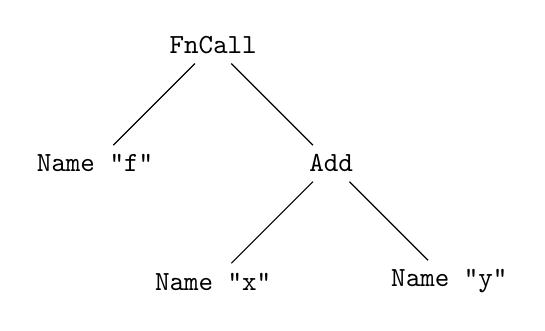
\begin{tikzpicture}[level distance=1.5cm,
    level 1/.style={sibling distance=3cm},
    level 2/.style={sibling distance=3cm}]
  \node{\texttt{FnCall}}
    child {node {\texttt{Name "f"}}}
    child {node {\texttt{Add}}
      child {node {\texttt{Name "x"}}}
      child {node {\texttt{Name "y"}}}
    };
\end{tikzpicture}
\end{center}

\vspace{0.5cm}

There are several different techniques of parsing, such as recursive descent and
LL. These methods often suffer from complex, unreadable code. However, Haskell's
type system allows me to use a different approach for parsing: parser
combinators. These allow you to use operators to combine simple parsers in
different ways to create complex ones. This technique of parsing is not without
issues - one of the main ones is that it is quite slow compared to conventional
techniques like recursive descent. However, the speed is still acceptable, and
their simplicity means that this is likely the technique I will use for parsing
my language.

The syntax of purely functional programming languages tends to be relatively
similar; they are mostly based off of either Haskell or Standard ML.
Haskell-like syntax looks like this:

\begin{verbatim}
  -- This is a comment
  foo :: Int -> Int  -- The type of "foo": it is a function from int to int
  foo x = x + 2      -- The definition of "foo": it adds 2 to its argument
\end{verbatim}

This is a very readable syntax, and has inspired other languages like OCaml.
However, it uses indentation for parsing; this can be quite complicated to do.
As such, for simplicity, I plan to change this syntax style slightly to allow
parsing without indentation. On the downside, this will make the syntax slightly
harder to read; however, it will simplify the parser greatly.

\subsection{Data types}

A more simple feature of Haskell is algebraic data types (ADTs). These are
datastructures which have multiple constructors, each containing some number of
values; for instance, a data type describing a list of integers could be
recursively defined in Haskell as follows: 

\begin{verbatim}
  data IntList = Cons Int IntList | Nil 
\end{verbatim}

This declaration specifies that an IntList either consists of the Cons
constructor applied to an Int and another IntList (representing the rest of the
list), or the Nil constructor applied to no arguments, which represents the
empty list. This feature is shared by non-lazy languages like OCaml and Standard
ML; it allows for a simple, intuitive, and safe representation of many data
structures. 

\subsection{Lazy evaluation}

Laziness is a relatively broad term in programming langauges; language like
Haskell provide purely lazy semantics, while some like OCaml allow you to opt-in
to laziness, and others like Perl 6 support laziness only in instances of
certain data structures (like lists). Here, we will be looking at a fully lazily
evaluated language, as in Haskell. This form of laziness can be incredibly
useful for defining recursive datastructures; for instance, the definition of an
infinite list in Haskell is simply as follows: 

\begin{verbatim}
  x = 1 : x 
\end{verbatim}

This definition works because the elements of x are only evaluated when they
need to be. 

\subsection{Type systems}

Another major feature of most functional languages is the type system.
Sophisticated type systems allow the programmer to specify very precise types
for values in the language; they act as a form of machine-checked documentation,
but also come with benefits like easy polymorphism.

Most ``interesting'' type systems are based on the lambda calculus, a theoretical
model for program execution (like Turing machines). There are three main type
systems to consider; the simply typed lambda calculus (hereafter referred to as
STLC for brevity), the Hindley-Milner type system, and System F.

\subsubsection{Simply-typed lambda calculus}

STLC is, as the name suggests, effectively the most simple possible type
system for the lambda calculus. It allows polymorphic types to be
constructed using function arrows, written \verb'->', and named type
variables. For example, the term \verb'\x. x' could be ascribed the type
\verb'a -> a', representing a function from a value of some type
\verb'a' to that same type. Similarly, \verb'\f. \x. f x' could be
ascribed the more complex type \verb'(a -> b) -> a -> b', representing a
function which converts a function \verb'a -> b' and a value \verb'a'
into a value \verb'b'. This is an incredibly helpful theoretical model;
however, it is not so useful in practical programming languages, since
for both efficiency and ease of code we want many, many more types than
just functions. Additionally, the simply-typed lambda calculus is
Turing-incomplete, making it impractical for use in a programming
language.

\subsubsection{Hindley-Milner typing}

The Hindley-Milner type system (sometimes referred to as Damas-Milner) extends
the STLC with the ability to work with types other than functions. This
is an incredibly popular type system for several reasons; the main one
is that type inference is completely decidable within this system.  This
means that given an expression with no type annotations (explicit pieces
of code informing the compiler of the type of expressions), the compiler
can always infer the most general (i.e.  polymorphic) type for an
expression by itself. This type system is used by the Haskell spec,
whose type system is effectively Hindley-Milner extended with
typeclasses. There also exists a relatively straightforward algorithm
for describing this type system, called Algorithm W. HM is proven to be
effectively as expressive as it is possible for a type system to be
whilst retaining decidability.

\subsubsection{System F}

System F is a more sophisticated type system, implemented by modern GHC's
dialect of Haskell. It extends the Hindley-Milner system with rank N types - in
layman's terms, ``nested polymorphism''. For instance:

\begin{verbatim}
  \f. (f 3, f "hi")
\end{verbatim}

This is a lambda which applies a function, given as its argument, to the values
3 and ``hi''. Because these values have different types, this program cannot be
expressed in the Hindley-Milner type system. These more complex types can be
beneficial in several areas of code (hence GHC's support for them); however,
they also greatly increase the complexity of the type system. Type inference
within System F is undecidable; this means it requires user-supplied type
annotations for inference to be successful. There is also no standard algorithm
for type checking and inference of System F expressions; there are many
competing methods of doing this, such as bidirectional type systems (e.g. the
one described in ``Practical type inference for arbitrary-rank types''; S. Peyton
Jones, D. Vytiniotis, S. Weirich, M. Shields; Microsoft Research). Due to this
complexity, and the relatively few benefits, I will likely not implement the
System F type system in any capacity; instead, I plan to implement the
Hindley-Milner system.

\subsubsection{Typeclasses}

Typeclasses are an extention to the Hindley-Milner (or System F) type system
which allow for increased polymorphism. An example of the motivation for these
is a sorting function; a comparison-based sorting function, under simple System
F, cannot be polymorphic. This is because it can not be applied to any type, but
rather only those which are ordered. Typeclasses are effectively a more powerful
version of interfaces as seen in OOP, and are Haskell's defining feature.
However, these complicate type inference and checking drastically, so while they
are a very helpful feature, they are not going to be a primary aim for this
project (although I may revisit them if I have time).

\subsection{Lazy evaluation}

In order to understand the implementation of laziness, we must first define what
``evaluation'' of an expression means. To do this, we define three ``forms'' of
expression; normal form (NF), head normal form (HNF), and weak head normal form
(WHNF). 

\begin{itemize}

  \item An expression in normal form is effectively fully evaluated. More
  specifically, an expression in NF is either a data constructor applied to
  arguments all in NF, or a lambda abstraction whose body is also in normal
  form. 

  \item An expression in head normal form is either a data constructor applied to
  arguments (which may be in any form), or a lambda abstraction whose body is
  in head normal form. 

  \item An expression in WHNF is either a data constructor applied to arguments
  (which may be in any form), or a lambda abstraction (whose body may be in
  any form). 

\end{itemize}

The most important of these ``forms'' is weak head normal form (WHNF). The way
evaluation actually occurs in a lazy language is through pattern matching, which
effectively allows you to deconstruct a type. For example, using the previously
defined IntList: 

\begin{verbatim}
  sum = \x -> case x of { Cons x xs -> x + sum xs; Nil -> 0 } 
\end{verbatim}

This defines 'sum' as a lambda (anonymous function) of one argument x. This
argument (which should be an IntList) is then deconstructed with a 'case'
expression; this looks at the constructor of x, and runs a different piece of
code depending on the constructor used. This case expression is the only way
evaluation occurs in most lazy languages. For this, we evaluate the expression
(which may be an unevaluated expression, known as a 'thunk') into weak head
normal form. This guarantees that, as long as the value is of the correct type,
the constructor in question will be evaluated, and can be matched against. 

\subsection{Objectives}

\begin{itemize}

  \item Create a parser for a Haskell-like functional programming syntax into an AST

  \item Implement inference and checking for the Hindley-Milner type system with ADTs
  using Algorithm W

  \item Convert this AST into a simpler, untyped IR language

  \item Convert this IR into AMD64 assembly (which supports lazy evaluation with
    thunks), using a low-level runtime written in C

  \item Implement a garbage collector to prevent memory leaks in written code

\end{itemize}

\end{document}
